\chapter{随机变量}

\begin{introduction}
    \item 离散与连续随机变量
    \item 一元与多元
    \item cdf, pmf, pdf
    \item 条件分布
    \item 独立随机变量
    \item 随机变量函数的分布
    \item 次序随机变量
\end{introduction}

在概率论中,主要关心$X$取值于数值集合$\mathcal{X}$中某个子集$B$的可能性, 即希望得到$\P(\{\omega\in\Omega : X(\omega) \in B\})$. 概率论不关心具体的样本点$\omega\in\Omega$, 将其记为$\{X \in B\} = X^{-1}(B)$. 由于$\P$定义在$\mathscr{F}$上, 故需$X^{-1}(B) \in \mathscr{F}$.

\begin{definition}[可测性]
    设所有值得关心的$B\subset \mathcal{X}$组成$\mathscr{F}_{\mathcal{X}}$, 且$\forall B \in \mathscr{F}_{\mathcal{X}}$都满足$\{X\in B\} \in \mathscr{F}$, 则称$X$为$\mathscr{F}/\mathscr{F}_{\mathcal{X}}$\textbf{可测的}. 当$\mathscr{F}_{\mathcal{X}}$不引起混淆时, 简记为关于$\mathscr{F}$\textbf{可测}, 写作$X \in \mathscr{F}$.
\end{definition}

由于原像保持交、并、补等集合运算, 且$\mathscr{F}$是$\sigma$代数, 可将$\mathscr{F}_{\mathcal{X}}$扩张为合适的最小的$\sigma$代数, 即$\sigma(\mathscr{F}_{\mathcal{X}})$, 因此可测映射的定义不妨\underline{只考虑$\mathscr{F}_{\mathcal{X}}$是$\sigma$代数}的情况.

\begin{definition}[随机变量]
    为了表示因随机性而变动的量, 称\underline{可测映射}(measurable mapping)
    \[ X : (\Omega,\mathscr{F},\P) \to (\mathcal{X},\mathscr{F}_{\mathcal{X}}), \quad \omega\in\Omega \mapsto X(\omega)\in\mathcal{X} \]
    为\textbf{随机元}(random element), 也称\textbf{随机变量}(random variable). 其中$\mathscr{F}_{\mathcal{X}}$
\end{definition}

由于只考虑$\mathscr{F}_{\mathcal{X}}$是$\sigma$代数的情况, 可将随机变量看作将原概率空间映射到新概率空间的方式. 新样本空间由\underline{Borel点集}构成, 对应的概率测度等于原像的.

\begin{remark}
    使用随机变量$X$时, 有两个可能的含义:
    \begin{itemize}
        \item $X$的(随机)取值
        \item $X$的分布
    \end{itemize}
\end{remark}

\begin{definition}[离散与连续随机变量]
    当$\mathcal{X}$是 (至多可数的) 离散点集, $\mathscr{F}_{\mathcal{X}}$由$\mathcal{X}$的所有子集组成, 则称其为\textbf{离散随机变量}(discrete random varible). 当随机变量$\mathcal{X} = \R^{n}$, 考虑$\mathscr{F}_{\mathcal{X}}$为$\left\{\prod_{i=1}^{n}(-\infty,x_{i}] : x_{1},\dots,x_{n}\in\R\right\}$生成的Borel代数(最小的$\sigma$代数), 则称其为\textbf{连续随机变量}(continuous random varible).
\end{definition}

\section{随机变量的分布}

\begin{definition}
    称随机元$X$诱导的\underline{概率测度}
    \[ \P\{X\in\bullet\},\ \bullet\in\mathscr{F}_{\mathcal{X}} \]
    为$X$的\textbf{概率分布}(distribution/law)
\end{definition}
\begin{remark}
    对于随机变量, 他的取值是随机的, 但他的分布是固定的
\end{remark}

\begin{definition}[单变量分布函数]
    一个函数$F : \R \to [0,1]$称为一个单变量分布函数,当其满足以下性质时:
    \begin{description}
        \item[单调性] $F(x_1)\le F(x_2) , \quad \forall x_1<x_2$
        \item[右连续性] $\lim_{x \to x_0^+}F(x)=F(x_0)$
        \item[有界性] $\lim_{n \to -\infty}F(x)=0, \quad \lim_{n \to \infty}F(x)=1$
    \end{description}
\end{definition}

\begin{property}
    $F(x)$最多只有可数个间断点
\end{property}

\begin{proposition}
    对每个分布$Q: \mathscr{B}_1 \to [0,1]$都存在唯一一个分布函数$F_Q : \R \to [0,1]$使得$F_Q(x)=Q[(-\infty,x]], \quad \forall x \in \R$成立。
\end{proposition}

\begin{proposition}
    对每个分布函数$F : \R \to [0,1]$都存在唯一一个分布$Q_F: \mathscr{B}_1 \to [0,1]$使得$Q_F[(-\infty,x]]=F(x), \quad \forall x \in \R$成立。
\end{proposition}

\begin{theorem}
    分布函数可以唯一决定概率分布, 即:
    \[ Q_{F_Q}=Q, \quad F_{Q_F}=F \]
    把随机变量$X$服从分布函数$F(x)$简记作$X \thicksim F(x)$
\end{theorem}

\begin{table}[h]
    \centering
    \begin{tabular}{|c|cc|}
        \hline
                                      & \multicolumn{1}{c|}{离散}                                 & 连续                        \\ \hline
        \multirow{3}{*}{一元随机变量} & \multicolumn{1}{c|}{概率质量函数(pmf)}                    & 概率密度函数(pdf)           \\ \cline{2-3}
                                      & \multicolumn{2}{c|}{累积分布函数(cdf)}                                                  \\ \cline{2-3}
                                      & \multicolumn{2}{c|}{矩母函数/特征函数(mgf/chf)}                                         \\ \hline
        \multirow{3}{*}{多元随机变量} & \multicolumn{1}{c|}{联合概率质量函数(joint pmf)}          & 联合概率密度函数(joint pdf) \\ \cline{2-3}
                                      & \multicolumn{2}{c|}{联合累积分布函数(joint cdf)}                                        \\ \cline{2-3}
                                      & \multicolumn{2}{c|}{联合矩母函数/特征函数(joint mgf/chf)}                               \\ \hline
    \end{tabular}
\end{table}

\begin{definition}[累积分布函数]
    此时$X = (X_{1},\dots,X_{n})^{\top}$的分布由(累积)\textbf{分布函数}(cumulative distribution function, c.d.f.)
    \[ F_{X}(x_{1},\dots,x_{n}) = \P\{X_{1}\leq x_{1},\dots, X_{n}\leq x_{n}\}, \quad x_{1},\dots,x_{n}\in\R. \]
    唯一刻画. 把随机变量$X$服从分布函数$F(x)$简记作$X \thicksim F(x)$
\end{definition}

\begin{figure}[h]
    \centering
    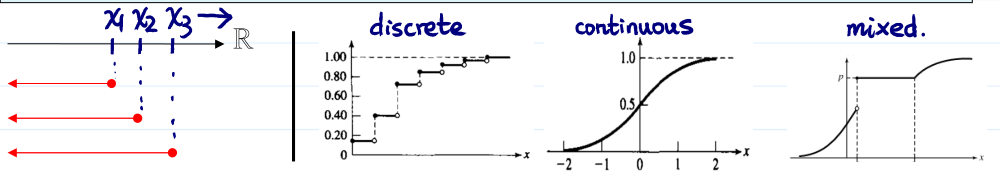
\includegraphics[width=0.8\textwidth]{image/cdf.png}
\end{figure}

\begin{definition}[概率质量函数]
    当且仅当函数$p(x)$满足下述条件时, 被称为\textbf{概率质量函数}(probability mass function, p.m.f.):
    \begin{itemize}
        \item $p(x)\ge 0$
        \item $\sum_{x \in \X}p(x)=1$
    \end{itemize}
\end{definition}

当$X$是离散型随机变量, 设$\mathscr{F}_{\mathcal{X}}$由$\mathcal{X}$的所有子集组成, 此时$X$的分布由
\[ p_{X}(x) = \P\{X=x\} = \P(\{\omega\in\Omega:X(\omega)=x\}), \quad x\in\mathcal{X} \]
唯一刻画. 其与分布函数间的关系为:
\begin{itemize}
    \item $F(x) = \sum_{t\le x}P(X=t)=\sum_{t\le x}p(t)$
    \item $p(x)=P(X=x)=F(x)-F(x-)$
\end{itemize}

\begin{definition}[概率密度函数]
    当且仅当函数$f(x)$满足下述条件时, 被称为\textbf{概率密度函数}(probability density function, p.d.f.):
    \begin{itemize}
        \item $f(x)\ge 0$
        \item $\int_{-\infty}^{\infty}f(x)=1$
    \end{itemize}
\end{definition}

当$X$是连续型随机变量, 且$F_{X} : \R^{n} \to [0,1]$可微(或者更一般地, \underline{绝对连续}), 此时$X$的分布由
\[ f_{X} := \frac{\partial^{n} F_{X}}{\partial x_{1} \cdots \partial x_{n}} \]
唯一刻画. 其与分布函数间的关系为:
\begin{itemize}
    \item $F(x) = \int_{-\infty}^x f(t)dt$
    \item $f(x)=\frac{d}{dx}F(x)$
\end{itemize}

\begin{remark}
    即使对于$f(x)>0$的$x$, $P(X=x)=x\int_{x}^x f(t)dt=0$, 即连续型随机变量在实轴上任意一点的概率测度为零. 概率密度函数$f(x)$代表的是在此位置上单位长度的概率, 可能是一个很大的值.
\end{remark}

\section{多元随机变量}

\begin{definition}[随机向量]
    若随机变量$X_1(\omega), X_2(\omega),\cdots , X_n(\omega)$定义在\underline{同一概率空间}$(\Omega,\mathscr{F},\P)$上, 则称
    \[ X(\omega) = (X_1(\omega), X_2(\omega),\cdots , X_n(\omega)) \]
    构成一个n维\textbf{随机向量},亦称n维随机变量.
\end{definition}

\begin{proposition}
    若$B_n$为$\R^n$上任一博雷尔点集,有
    \[ \{ X(\omega) \in B_n \} \in \mathscr{F} \]
\end{proposition}

\begin{definition}
    称n元函数
    \[ F(x_1,x_2, \cdots , X_n)=\P \{ X_1(\omega)<x_1, X_2(\omega)<x_2,\cdots , X_n(\omega)<x_n \} \]
    为随机向量$X(\omega)$的\textbf{联合分布函数}(joint cdf).
\end{definition}

当$n=2$时,有
\begin{equation}\label{equ:2dim_Prob}
    \P((a_1,b_1)\le X < (a_2,b_2))=F(b_1,b_2)-F(a_1,b_2)-F(b_1,a_2)+F(a_1,a_2)
\end{equation}

\begin{property}
    多元分布函数的一些性质:
    \begin{enumerate}
        \item 单调性:关千每个变元是单调不减函数;
        \item \begin{align*}
                  F(x_1,x_2, \cdots, -\infty, \cdots, X_n)=0 \\
                  F(+\infty,+\infty, \cdots, , +\infty)=1
              \end{align*}
        \item 关于每个变元右连续.
        \item 在二元场合,还应该有:对任意$ a_1 <b,,a_2<b_2$ ,都有
              \[ F(b_1,b_2)-F(a_1,b_2)-F(b_1,a_2)+F(a_1,a_2)\ge 0   \]
    \end{enumerate}
\end{property}

为保证\ref{equ:2dim_Prob}式中的概率的非负性,性质4是必须的,而且由性质4可以推出单调性,但存在着反例说明,由单调性并不能保证性质4的成立(见习题 12) .这是多元场合与一元场合的不同之处.

\subsection{边际分布}

\begin{definition}
    对于多维随机变量$X$, 只考虑其中一个分量的分布时, 称其为$X$的\textbf{边际分布或边缘分布}. 对于分量$X_i$, 其\textbf{边缘分布函数}(marginal cdf)为:
    \[ F_{X_i}(x_i) = \P\{ X_i \le x_i \} = F(\infty,\cdots , x_i ,\cdots ,\infty)\]
\end{definition}

\subsection{条件分布}

\begin{definition}\label{def:cond_dist}
    对一切使 $P\left(Y=y_{j}\right)=p_{ \cdot j}=\sum_{i=1}^{+\infty} p_{i j}>0$ 的 $y_j$, 称
    \[ p_{i | j}=P\left(X=x_{i} | Y=y_{j}\right)=\frac{P\left(X=x_{i}, Y=y_{j}\right)}{P\left(Y=y_{j}\right)}
        =\frac{p_{i j}}{p_{\cdot j}}, \quad i=1,2, \ldots \]
    为给定 $Y=y_j$ 条件下 $X$ 的条件分布列. 若$p_X(x)=0$, 则定义其为0.
\end{definition}

设二维连续随机变量 $(X,Y)$ 的联合密度函数为 $p(x,y)$, 边际密度函数为 $p_X(x),p_Y(y)$.

在离散随机变量场合, 其条件分布函数为 $P(X\leq x|Y=y)$. 但是, 因为连续随机变量取某个值的概率为零, 即 $P(Y=y)=0$, 所以无法用条件概率直接计算 $P(X\leq x|Y=y)$, 一个很自然的想法是: 将 $P(X\leq x|Y=y)$ 看成是 $h\to 0$ 时 $P(X\leq x|y\leq Y\leq y+h)$ 的极限, 即
\begin{align*}
    P(X \leq  x | Y=y) & =\lim _{h \to 0} P(X \leq  x | y \leq  Y \leq  y+h)                                                  \\
                       & =\lim _{h \to 0} \frac{P(X \leq  x, y \leq  Y \leq  y+h)}{P(y \leq  Y \leq  y+h)}                    \\
                       & =\lim _{h \to 0} \frac{\int_{-\infty}^{x} \int_{y}^{y+h} p(u, v) dv du}{\int_{y}^{y+h} p_{Y}(v) dv}  \\
                       & =\lim _{h \to 0} \frac{\int_{-\infty}^{x} \left\{ \frac{1}{h} \int_{y}^{y+h} p(u, v) dv \right\} du}
    {\frac{1}{h} \int_{y}^{y+h} p_{Y}(v) dv}.
\end{align*}
当 $p_Y(y),p(x,y)$ 在 $y$ 处连续时, 由积分中值定理可得
\begin{align*}
     & \lim _{h \to 0} \frac{1}{h} \int_{y}^{y+h} p_{Y}(v) dv=p_{Y}(y), \\
     & \lim _{h \to 0} \frac{1}{h} \int_{y}^{y+h} p(u, v) dv=p(u, y).
\end{align*}
所以
\[ P(X \leq x | Y=y)=\int_{-\infty}^{x} \frac{p(u, y)}{p_{Y}(y)} du \]
至此, 我们可以定义连续随机变量的条件分布如下.

\begin{definition}
    对一切使 $p_Y(y)>0$ 的 $y$, 给定 $Y=y$ 条件下 $X$ 的\textbf{条件分布函数}\index{T!条件分布函数}和
    \textbf{条件密度函数}\index{T!条件密度函数}分别为
    \begin{align*}
         & F(x | y)=\int_{-\infty}^{x} \frac{p(u, y)}{p_{Y}(y)} du, \\
         & p(x | y)=\frac{p(x, y)}{p_{Y}(y)}.
    \end{align*}
    同理对一切使 $p_Y(y)>0$ 的 $x$, 给定 $X=x$ 条件下 $Y$ 的条件分布函数和条件密度函数分别为
    \begin{align*}
         & F(y | x)=\int_{-\infty}^{y} \frac{p(x, v)}{p_{X}(x)} dv \\
         & p(y | x)=\frac{p(x, y)}{p_{X}(x)}.
    \end{align*}
\end{definition}

\begin{remark}
    对于每一个\underline{固定的$x$}, $p_{Y|X}(y|x)$是一个关于$y$的概率质量函数; $f_{Y|X}(y|x)$是一个关于$y$的概率密度函数
\end{remark}

与概率三定理的对应:
\begin{description}
    \item[乘法法则] $p_{XY}(x,y)=p_{Y|X}(y|x)p_{X}(x), \quad f_{XY}(x,y)=f_{Y|X}(y|x)f_{X}(x)$
    \item[全概率公式] $p_{Y}(y)=\sum_{x}p_{Y|X}(y|x)p_{X}(x), \quad f_{Y}(y)=\int^{+\infty}_{-\infty}f_{Y|X}(y|x)f_{X}(x)dx$
    \item[Bayes原理]  $p_{X|Y}(x|y)=\frac{p_{Y|X}(y|x)p_{X}(x)}{\sum_{x}p_{Y|X}(y|x)p_{X}(x)}, \quad f_{X|Y}(x|y)=\frac{f_{Y|X}(y|x)f_{X}(x)}{\int^{+\infty}_{-\infty}f_{Y|X}(y|x)f_{X}(x)dx}$
\end{description}

\subsection{独立}

\begin{definition}[独立随机变量]
    若随机变量$X(\omega) = (X_1(\omega), X_2(\omega),\cdots , X_n(\omega))$联合分布函数可分解成各分量边缘分布函数的乘积, 即:
    \[ F(x_1,x_2,\cdots ,x_n) = F_{X_1}(x_1)F_{X_2}(x_2)\cdots F_{X_n}(x_n) , \quad \forall x_1,x_2,\cdots ,x_n \in \R \]
    则称随机变量$X$各分量相互\textbf{独立}
\end{definition}

\begin{remark}
    对于一般的多元随机变量, 其各分量边缘分布不足以描述联合分布的情况. 但若其各分量独立则可以.
\end{remark}

\begin{theorem}\label{thm:indep_cmf}
    对于连续情况:
    \begin{align*}
                        & F(x_1,x_2,\cdots ,x_n) = F_{X_1}(x_1)F_{X_2}(x_2)\cdots F_{X_n}(x_n) \\
        \Leftrightarrow & f(x_1,x_2,\cdots ,x_n) = f_{X_1}(x_1)f_{X_2}(x_2)\cdots f_{X_n}(x_n)
    \end{align*}
    对于离散情况:
    \begin{align*}
                        & F(x_1,x_2,\cdots ,x_n) = F_{X_1}(x_1)F_{X_2}(x_2)\cdots F_{X_n}(x_n) \\
        \Leftrightarrow & p(x_1,x_2,\cdots ,x_n) = p_{X_1}(x_1)p_{X_2}(x_2)\cdots p_{X_n}(x_n)
    \end{align*}
\end{theorem}

\section{随机变量的函数}

在统计学中,常需要转化原始数据以获取其中信息, 由此引出了研究随机变量的函数的需要.

\begin{definition}[可测函数]
    设$y =g(x)$是$\R$到$\R$上的一个映照,若对于一切$\R$中的Borel点集$B_1$均有
    \[\left\{ x:g(x) \in B_1 \right\} \in \mathcal{B}_1 \]
    其中$\mathcal{B}_1$为$\R$上Borel $\sigma$域,则称$g(x)$是一元博雷尔函数, 也称为一元\textbf{可测函数}
\end{definition}

\begin{theorem}[事件法]
    设$Y=g(X)$是随机向量$X=(X_1,X_2,\cdots ,X_n)$的函数, 则$Y$的分布由$X$的分布通过下式决定:
    \[ \P\{Y \in B\} = \P\{X \in A\}, \quad A=\{ \omega |g(X(\omega))\in B\} \]
\end{theorem}

此法是其他方法的基础, 但使用不便, 常用于离散随机变量.

\begin{example}\label{exp:sum_of_pmf}
    已知随机变量$X,Y$的联合概率质量函数为$p(x,y)$, 求$Z=X+Y$的分布
\end{example}

\begin{solution}
    \[ p_Z=P(Z=z)=P(X+Y=z)=\sum_{x=-\infty}^{\infty}p(x, z-x) \]
    若$X,Y$独立,则$p_Z(z)=\sum_{-\infty}^{\infty}p_X(x)p_Y(z-x)dx$, 为$p_X$与$p_Y$的卷积
\end{solution}

\begin{theorem}[]
    若随机变量$X,Y$独立, 则其变换$Z=g(X), W=h(Y)$也独立.

    泛化情况:若随机向量$\{X\}_n$各分类独立, 则其变换$\{Y\}_n=g(\{X\}_n)$各分类也独立.
\end{theorem}

\begin{proof}
    %TODO: 待补
\end{proof}

\subsection{分布函数法}

通过下式获取随机变量的函数的分布:
\[ F_Y(y)=\begin{cases}
        \int_{A_y}f_X(x)dx \\
        \sum_{x \in A_y}p_X(x)
    \end{cases} , \quad A_y=\{ x|g(x)\le y \}
\]

对每一个变换分别运用上式则可得到向量函数的分布.

\begin{example}
    已知随机变量$X$的概率密度函数$f_X(x)$与分布函数$F_X(x)$, 求$Y=X^2$的分布
\end{example}

\begin{solution}
    \[ F_Y(y)=P(Y\le y)=P(-\sqrt{y}<X\le \sqrt{y})+P(X=\sqrt{y}=F_X(\sqrt{y})-F_X(-\sqrt{y}))+0 \quad y\ge 0\]

    \begin{align*}
        f_Y(y) =\frac{d}{dy}F_Y(y) & =\frac{d}{dy}F_X(\sqrt{y}) -\frac{d}{dy}F_X(\sqrt{y})                 \\
                                   & =f_X(\sqrt{y})\frac{1}{2\sqrt{y}} -f_X(-\sqrt{y})\frac{-1}{2\sqrt{y}} \\
                                   & =\frac{1}{2\sqrt{y}}(f_X(\sqrt{y})+f_X(-\sqrt{y}))
    \end{align*}
\end{solution}

\begin{example}\label{exp:sum_of_pdf}
    已知随机变量$X,Y$的联合概率密度函数$f(x,y)$, 求$Z=X+Y$的分布
\end{example}

\begin{solution}
    \[ F_Y(y)=P(Y\le y)=P(-\sqrt{y}<X\le \sqrt{y})+P(X=\sqrt{y}=F_X(\sqrt{y})-F_X(-\sqrt{y}))+0 \quad y\ge 0\]

    \begin{align*}
        F_Z(z) & =P(Z\le z)=P(X+Y\le z)                                               \\
               & =\iint _{x+y\leqslant z}f(x,y)dxdy                                   \\
               & =\int_{-\infty}^{+\infty}\int_{-\infty}^{z-x}f(x,y)dxdy              \\
               & =\int_{-\infty}^{z}\int_{-\infty}^{\infty}f(x,v-x)dxdv, \quad y= v-x
    \end{align*}

    \[ f_Z(z)=\frac{d}{dz}F_Z(z)=\int_{-\infty}^{\infty}f(x,z-x)dx \]

    若$X,Y$独立,则$f_Z(z)=\int_{-\infty}^{\infty}f_X(x)f_Y(z-x)dx$, 为$f_X$与$f_Y$的卷积, 与\ref{exp:sum_of_pmf}类似
\end{solution}

\begin{example}
    已知随机变量$X,Y$的联合概率密度函数$f(x,y)$, 求$Z=\frac{Y}{X}$的分布
\end{example}

\begin{solution}
    \[ Q_{z}=\{(x, y): y / x \leq z\}=\{(x, y): x<0, y \geq z x\} \cup\{(x, y): x>0, y \leq z x\} \]
    \begin{align*}
        F_{Z}(z) & =\iint_{Q_{z}} f(x, y) d x d y=\int_{-\infty}^{0} \int_{x z}^{\infty}+\int_{0}^{\infty} \int_{-\infty}^{x z} f(x, y) d y d x \\
                 & =\int_{-\infty}^{0} \int_{z}^{-\infty}+\int_{0}^{\infty} \int_{-\infty}^{z} x f(x, x v) d v d x \quad(\text{set} y=x v)      \\
                 & =\int_{-\infty}^{0} \int_{-\infty}^{z}(-x) f(x, x v) d v d x+\int_{0}^{\infty} \int_{-\infty}^{z} x f(x, xv) dvdx            \\
                 & =\int_{-\infty}^{z} \int_{-\infty}^{\infty}|x| f(x, xv) dxdv
    \end{align*}

    \[ f_Z(z)=\frac{d}{dz}F_Z(z)=\int_{-\infty}^{\infty}|x|f(x,xz)dx \]
\end{solution}

\subsection{Copula}\label{subsec:Copula}
\begin{definition}
    设\underline{连续型}实值随机变量$X$有分布函数$F$, 易见$F$在$\overline{\R}=[-\infty,+\infty]$上从$0$递增到$1$. 定义相应的\textbf{分位数函数}(quantile function)为
    \[ F^{-1}(p) := \inf\{x\in\R:F(x)\ge p\}, \quad p \in [0,1]. \]
\end{definition}
\begin{remark}
    当$F$严格递增时, 这与一般的反函数定义相同.
\end{remark}

\begin{theorem}
    设\underline{连续型}实值随机变量$X$有分布函数$F$, 则$F(X) \sim \mathrm{Uniform}([0,1])$
\end{theorem}

\begin{proof}
    \[ \P\{F(X)\le p\} = \P\{X\le F^{-1}(p)\} = F(F^{-1}(p)) =p, \quad \forall p \in [0,1]. \]
\end{proof}

\begin{theorem}\label{thm:pseudo_random_generation}
    设\underline{连续型}实值随机变量$X$有分布函数$F$, 且设$U\sim\mathrm{Uniform}([0,1]) $, 则$ F^{-1}(U) \overset{d}{=} X$, 其中$\overset{d}{=}$表示分布相同(equal in distribution).
\end{theorem}

\begin{theorem}[Sklar定理]
    考虑多个\underline{连续型}实值随机变量$X_{1},\dots,X_{k}$, 记$X_{i}$的分布函数为$F_{i}$. 我们称$(F_{1}(X_{1}),\dots,F_{k}(X_{k}))$的分布函数$C : [0,1]^{k} \to [0,1]$为相应的\textbf{Copula}, 适合
    \[ C(F_{1}(x_{1}),\dots,F_{k}(x_{k})) = \P\{X_{1}\le x_{1},\dots,X_{k}\le x_{k}\}, \quad \forall x_{1},\dots,x_{k} \]
    这个结果称为\textbf{Sklar定理}
\end{theorem}


这个结果, 在金融统计中有颇多应用. 稍作诠释的话, Copula提取了变量间的\emph{相关性}, 通过粘合\emph{边际}能够恰好地表示\emph{总体}.
人们可以构造各种各样的Copula, 对真实世界进行建模.

\subsection{概率密度函数法}

\begin{theorem}
    设连续随机变量$X$的概率密度函数为$f_X(x)$. 令$Y=g(X)$, 其中$g$为可微函数, 且严格单调, 则当$y=g(x)$有定义时:
    \[ f_Y(y)=f_X(g^{-1}(y))\left| \frac{dg^{-1}(y)}{dy} \right|  \]
    否则为$0$

    若$g$为分段单调函数, 则\underline{分段}计算上是结果, 再进行相加
\end{theorem}

\begin{theorem}
    设连续随机向量$\mathbf{X}$的概率密度函数为$f_\mathbf{X}(\mathbf{x})$. 令$\mathbf{Y}=\mathbf{g}(\mathbf{X})$, 其中$\mathbf{g}$为双射, 定义其逆函数为:
    \[ \mathbf{x}=\mathbf{g}^{-1}(\mathbf{y})=\mathbf{w}(\mathbf{y}) \]
    若$\mathbf{w}$存在连续偏导数, 则当$\mathbf{Y}=\mathbf{g}(\mathbf{X})$有定义时:
    \[ f_\mathbf{Y}(\mathbf{y})=f_\mathbf{X}(\mathbf{g}^{-1}(\mathbf{y}))\left| \frac{\partial \mathbf{w}}{\partial \mathbf{y}} \right|  \]
    否则为$0$
\end{theorem}

\begin{remark}
    若$\mathbf{Y}$的维数$k$小于$\mathbf{X}$的维数$n$, 可增补$n-k$维的函数$\mathbf{Z}=\mathbf{h}(\mathbf{X})$, 使得$(\mathbf{Y},\mathbf{Z})$满足条件, 再通过积分获取$\mathbf{Y}$的概率密度函数.
\end{remark}

\begin{example}
    已知随机变量$X_1,X_2$的联合概率密度函数$f(x_1,x_2)$, 求$Y_1=\frac{X_2}{X_1}$的分布
\end{example}

\begin{solution}
    令$Y_{2}=X_{1}$, 则:
    \begin{align*}
        x_{1} & =y_{2}\equiv w_{1}(y_{1}, y_{2})       \\
        x_{2} & =y_{1} y_{2}\equiv w_{2}(y_{1}, y_{2})
    \end{align*}
    \[ \frac{\partial w_{1}}{\partial y_{1}}=0, \frac{\partial w_{1}}{\partial y_{2}}=1, \frac{\partial w_{2}}{\partial y_{1}}=y_{2}, \frac{\partial w_{2}}{\partial y_{2}}=y_{1}\]
    \[ J=\left|\begin{array}{cc}0 & 1 \\ y_{2} & y_{1}\end{array}\right|=-y_{2}\]
    所以:
    \[ f_{Y_1 Y_2}(y_1, y_2)=f_{X_1 X_2}(y_{2}, y_{1} y_{2})\left|y_2\right| \]
    \begin{equation}
        f_{Y_1}(y_1)=\int_{-\infty}^{\infty} f_{Y_{1} Y_{2}}\left(y_{1}, y_{2}\right) d y_{2}=\int_{-\infty}^{\infty} f_{X_{1} X_{2}}\left(y_{2}, y_{1} y_{2}\right)\left|y_{2}\right| d y_{2}
        \label{equ:quotient_of_variable}
    \end{equation}
    \[  \]
\end{solution}

\begin{proposition}
    若随机向量$\mathbf{X}=(X_1,\cdots ,X_n)$各分类相互独立, 则其各分量的函数$\mathbf{Y}=(g_1(X_1),\cdots ,g_n(X_n))$也相互独立
\end{proposition}
\begin{proof}

\end{proof}

\subsection{矩母函数法}

\subsection{次序统计量}

\begin{definition}
    设$X_1,X_2,\dotsc,X_n$为随机变量, 将其按大小排序后记为$X_{(1)}\le X_{(2)} \le  \cdots \le X_{(n)}$, 则将$x_{(i)}$称为该样本的第$i$个\textbf{次序统计量}. 其中
    \begin{itemize}
        \item \textbf{最小次序统计量}定义为:$X_{(1)}=\min\{x_1,\dotsc,x_n\}$
        \item \textbf{最大次序统计量}定义为:$X_{(n)}=\max\{x_1,\dotsc,x_n\}$
        \item \textbf{极差}定义为:$R=X_{(n)}-X_{(1)}$
        \item 第$i$个\textbf{间差}定义为:$S_i=X_{(i)}-X_{(i-1)}$
    \end{itemize}
\end{definition}

\begin{remark}
    虽然$X_1,X_2,\dotsc,X_n$独立, 但其次序统计量一般不独立
\end{remark}

\begin{example}
    若$X_1,X_2,\dotsc,X_n$独立同分布, 求$X_{(1)}$与$X_{(n)}$的分布
\end{example}

\begin{solution}
    \begin{align*}
        F_{X_{(n)}}(x) & =P(X_{(n)} \leq x)=P(X_{1} \leq x, \ldots, X_{n} \leq x) \\
                       & =P(X_{1} \leq x) \cdots P(X_{n} \leq x)                  \\
                       & =[F(x)]^{n}                                              \\
        f_{X_{(n)}}(x) & = \frac{d}{dx}F_{X_{(n)}}(x)                             \\
                       & =nf(x)[F(x)]^{n-1}
    \end{align*}

    \begin{align*}
        1-F_{X_{(1)}}(x) & =P(X_{(1)}>x)=P(X_{1}>x, \ldots, X_{n}>x) \\
                         & =P(X_{1}>x)\cdots P(X_{n}>x)              \\
                         & =[1-F(x)]^{n}                             \\
        f_{X_{(1)}}(x)   & = \frac{d}{dx}F_{X_{(1)}}(x)              \\
                         & =nf(x)[1-F(x)]^{n-1}
    \end{align*}
\end{solution}

\begin{theorem}
    第$i$个\textbf{次序统计量}的概率密度函数为:
    \[ f_{X_{(k)}} = C(n;1,k-1,n-k)f(x)[F(x)]^{k-1}[1-F(x)]^{n-k}  \]
\end{theorem}

\begin{figure}[!ht]
    \centering
    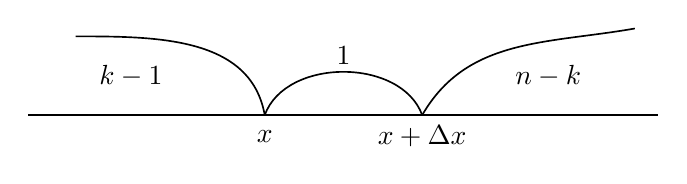
\begin{tikzpicture}[semithick]
        \draw(-4,0)--(4,0);\coordinate(a)at(-1,0);\node[below=2pt]at(a){$x$};
        \coordinate(b)at(1,0);\node[below]at(b){$x+\Delta x$};
        \draw[out=100,in=0](a)to(-3.4,1);
        \draw[out=70,in=110](a)to(b);
        \node at(0,0.75){$1$};\node at(-2.7,0.5){$k-1$};
        \draw[out=60,in=190](b)to(3.7,1.1);
        \node at(2.6,0.5){$n-k$};
    \end{tikzpicture}
    \caption{$X_{(k)}$取值的示意图}
\end{figure}

\begin{theorem}
    次序统计量$(x_{(i)},x_{(j)})(i<j)$的联合分布密度函数为
    \begin{align*}
        p_{ij}(y,z)=\frac{n!}{(i-1)!(j-i-1)!(n-j)!}[F(y)]^{i-1}[F(z)-F(y)]^{j-i-1} &   \\
        \cdot[1-F(z)]^{n-j}p(y)p(z),\quad y\leq z                                  & ,
    \end{align*}
\end{theorem}

\begin{proof}
    对正$\Delta y,\Delta z$以及$y<z$,事件``$x_{(i)}\in(y,y+\Delta y],x_{(j)}\in(z,z+\Delta z]$''可以表示为``容量为$n$的样本$x_1,\dotsc,x_n$中有$i-1$个观测值小于等于$y$,一个落入区间$(y,y+\Delta y],j-i-1$个落入区间$(y+\Delta y,z]$,一个落入区间$(z,z+\Delta z]$,而余下$n-j$个大于$z+\Delta z$''(见图~\ref{fig:5.3.6} ).
    \begin{figure}[!ht]
        \centering
        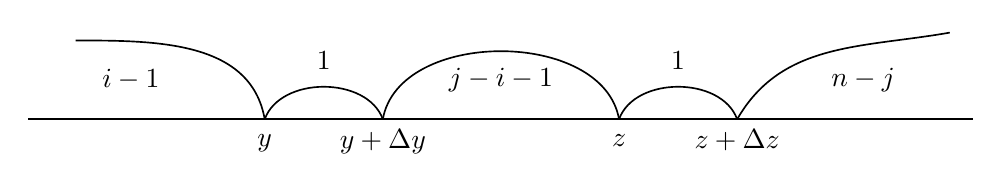
\begin{tikzpicture}[semithick]
            \draw(-6,0)--(6,0);
            \coordinate(a) at(-3,0);\coordinate(b)at(-1.5,0);
            \coordinate(c)at(1.5,0);\coordinate(d)at(3,0);
            \node[below=2pt]at(a){$y$};\node[below]at(b){$y+\Delta y$};
            \node[below=2pt]at(c){$z$};\node[below]at(d){$z+\Delta z$};
            \draw[out=100,in=0](a)to(-5.4,1);
            \draw[out=70,in=110](a)to(b);\draw[out=70,in=110](c)to(d);
            \node at(-2.25,0.75){$1$};\node at(-4.7,0.5){$i-1$};
            \draw[out=60,in=190](d)to(5.7,1.1);
            \node at(4.6,0.5){$n-j$};\node at(0,0.5){$j-i-1$};
            \draw[out=80,in=100](b)to(c);
            \node at(2.25,0.75){$1$};
        \end{tikzpicture}
        \caption{$x_{(i)}$与$x_{(j)}$取值的示意图}\label{fig:5.3.6}
    \end{figure}
\end{proof}
\begin{example}
    若$X_1,X_2,\dotsc,X_n$独立同分布, 求$R=X_{(n)}-X_{(1)}$的分布
\end{example}

\begin{solution}
    \[ f_{X_{(1)}X_{(n)}}(s,t)=n(n-1)f(s)f(t)[F(t)-F(s)]^{n-2}\mathbb{I}(s\le t) \]
    \[ f_R(r)=\mathbb{I}(r>0)\int_{-\infty}^{\infty}f_{X_{(1)}X_{(n)}}(s,s+r)ds \]
\end{solution}